\title{
    \begin{center}
    \Huge
    \textsc{The\\ Count of Monte-Cristo}
    \end{center}
}

\preauthor{\begin{center}}
\author{
    \MakeUppercase{
    {\tiny by}
    \\\vskip 2em
    {\Huge Alexandre Dumas}
    \\\vskip 3em
    {\tiny With nearly five hundred illustrations from designs by G. Staal, J. A. Beauce, and other
    eminent French artists}
    \\\vskip 5em
    {\normalsize \textsc{Vol. IV}}
}}
\postauthor{\end{center}}
\predate{\begin{center}}
\date{
\vfill
1888}
\postdate{\end{center}

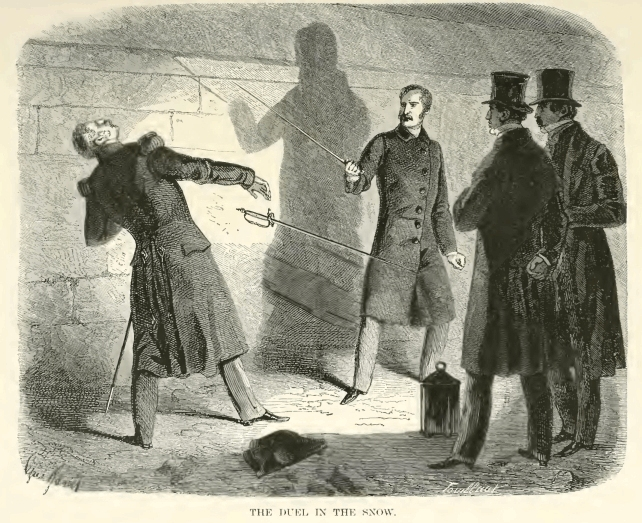
\includegraphics[width=0.75\textwidth]{40012m}

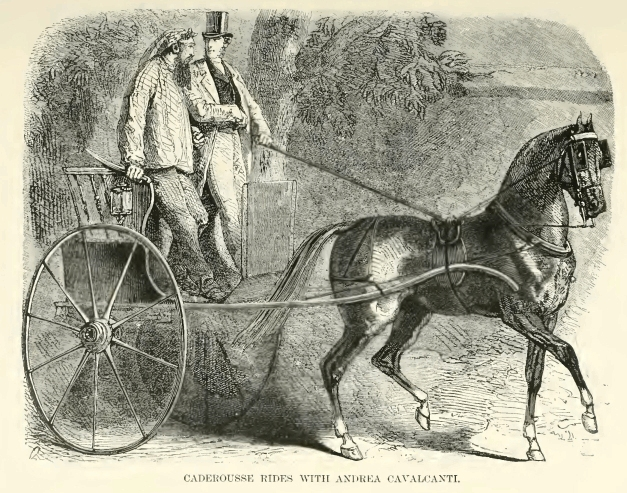
\includegraphics[width=0.75\textwidth]{40020m}
}

\maketitle
